\documentclass{SBCbookchapter}
\usepackage[utf8]{inputenc}
\usepackage[T1]{fontenc}
\usepackage[brazilian]{babel}
\usepackage{graphicx}
\usepackage[brazilian]{backref}	 % Paginas com as citações na bibl
\usepackage[alf]{abntex2cite}	% Citações padrão ABNT

% Figures
\usepackage[dvipsnames]{xcolor}
\usepackage{graphicx}
\usepackage{subcaption}

\usepackage{amsmath}

\usepackage{todonotes}

\author{Márcio Castro, Pedro H. Penna e Alyson D. Pereira\\
\textit{Departamento de Informática e Estatística (INE)}\\
\textit{Universidade Federal de Santa Catarina (UFSC)}
}
\title{Desenvolvimento de Aplicações Paralelas Eficientes com OpenMP}

% Fragmento de Código
\usepackage{listings}
\renewcommand{\lstlistingname}{Código}

\lstset{
  belowcaptionskip=1\baselineskip,
  breaklines=true,
  frame=L,
  xleftmargin=\parindent,
  numbers=left,
  stepnumber=1,
  language=C,
  tabsize=4,
  showstringspaces=false,
  basicstyle=\scriptsize\ttfamily,
  otherkeywords={
  	pragma,
	omp,
	parallel,
	num\_threads,
	schedule,
	reduction,
	private,
	shared,
	task,
	taskwait,
	single,
	nowait
  },
  keywordstyle=\color{blue},
  commentstyle=\itshape\color{gray},
  identifierstyle=\color{black},
  stringstyle=\color{purple},
}

\begin{document}
\maketitle

\begin{resumo}
Resumo aqui.
\end{resumo}

\section{Introdução}

	Durante as três últimas décadas, os avanços da tecnologia de
	semicondutores e de arquiteturas de computadores permitiram que o
	desempenho de um único processador fosse aumentado com uma taxa anual de
	40\% à 50\% \cite{LARUS08}. Porém, a dissipação de calor do crescente
	número de transistores em um único \emph{chip} começou a limitar o
	aumento da frequência dos processadores. Devido à esse fato, grande
	parte da indústria de semicondutores está agora investindo na produção
	de processadores com diversos núcleos de processamento
	(\emph{multicores}).

	De fato, processadores \emph{multicore} são largamente utilizados nos
	dias de hoje para a Computação de Alto Desempenho \cite{Asanovic09}.
	Porém, observa-se nessas arquiteturas uma grande disparidade entre o
	alto crescimento do número de \emph{cores} por processador e o baixo
	número de conexões entre processadores e o restante dos dispositivos.
	Essa crescente disparidade faz com que o tempo de acesso a um dado
	armazenado na memória seja muito maior que o tempo necessário para
	processá-lo, o que conduz ao conhecido ``\emph{memory wall problem}''
	\cite{McKee-MemWall:2004}. Esse problema é atenuado atualmente através
	do uso de uma hierarquia de memórias \emph{cache} entre os processadores
	e a memória principal, o que permite um acesso mais rápido aos dados e
	melhora o desempenho global.

	A tendência atual da construção de arquiteturas paralelas do tipo
	\emph{multicore} é de um crescimento contínuo do número de \emph{cores},
	resultando em arquiteturas compostas por dezenas ou até mesmo milhares
	de cores. Essa tendência é confirmada pelo \emph{website}
	TOP500\footnote{\url{http://www.top500.org}} (Figura~\ref{fig:top500}),
	o qual provê um ranking atualizado dos 500 supercomputadores mais
	poderosos do mundo. Nessas arquiteturas o problema de escalabilidade é
	ainda maior, pois centenas ou milhares de processos (ou \emph{threads})
	em execução simultânea disputam acesso a diversos recursos
	compartilhados como por exemplo \emph{cores}, memória principal,
	memórias \emph{cache}, entre outros.

	\begin{figure}[t]
		\centering
		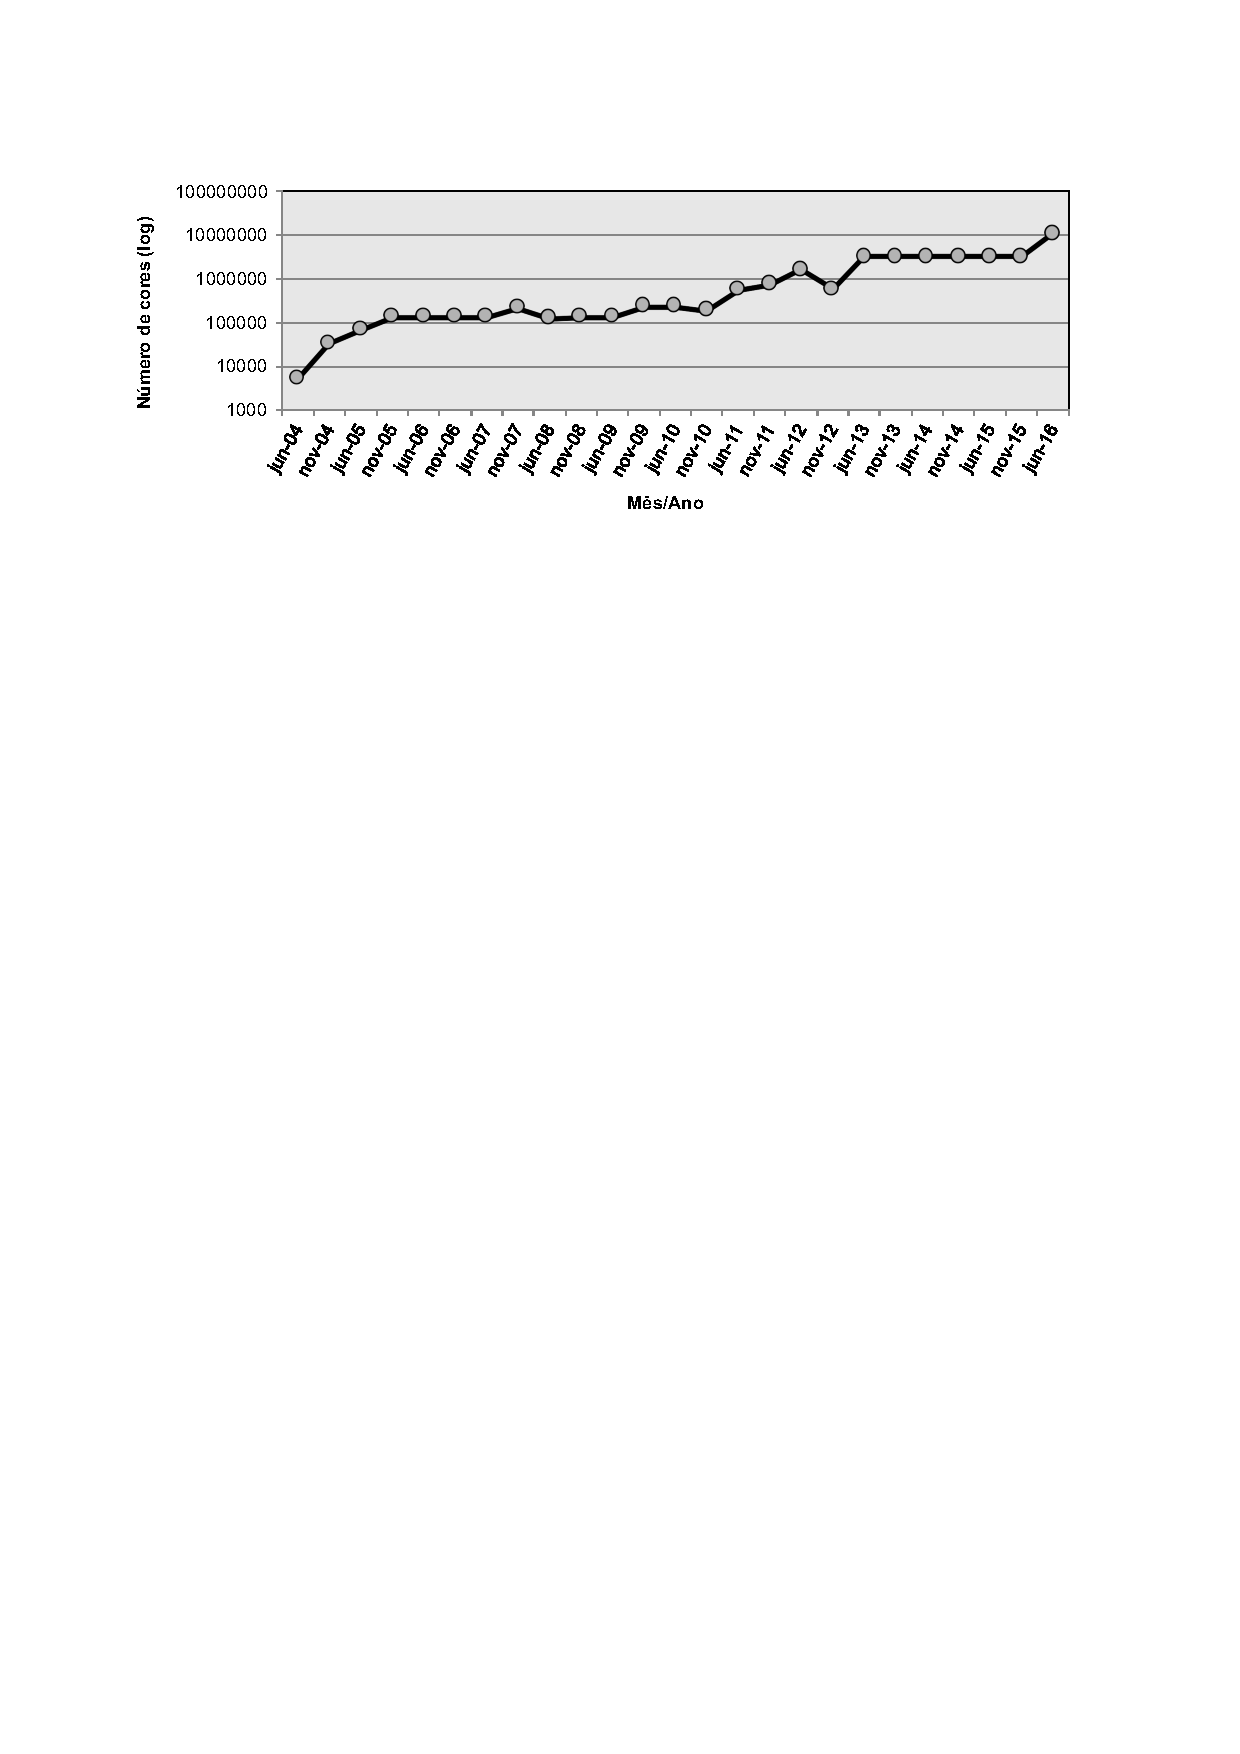
\includegraphics[width=13cm, height=!]{img/cores-top500.pdf}
		\caption{Número total de núcleos de processamento (\emph{cores}) dos
		supercomputadores mais poderosos relacionados na lista TOP500.}
		\label{fig:top500}
	\end{figure}

	O desenvolvimento de aplicações paralelas eficientes é um requisito
	obrigatório para que seja possível utilizar todo o potencial dessas.
	Para atingir esse objetivo é necessário o uso de modelos de programação
	paralela. Idealmente, esses modelos devem oferecer um nível de abstração
	alto aos desenvolvedores. Ao mesmo tempo, eles devem fornecer mecanismos
	eficientes para a criação, gerenciamento e orquestração de
	\textit{threads} ou processos.

	Nesse capítulo será apresentado um dos modelos de programação paralela
	muito utilizados na academia e na indústria denominado OpenMP. Esse
	modelo oferece diretivas de compilação que permitem realizar a
	paralelização de trechos de código de maneira transparente. O OpenMP
	oferece uma Interface de Programação de Aplicações (\textit{Application
	Programming Interface} -- API) bastante completa para paralelização de
	aplicações para arquiteturas de memória compartilhada. Nesse tipo de
	arquitetura, diversos processadores ou \textit{cores} tem acesso a uma
	memória principal compartilhada em um único espaço de endereçamento.
	A Figura~\ref{fig:uma-numa} apresenta uma visão geral de duas arquiteturas
	de memória compartilhada.

			\begin{figure}[t]
				\captionsetup[subfigure]{justification=centering}
				\centering
					\begin{subfigure}{0.45\linewidth}
						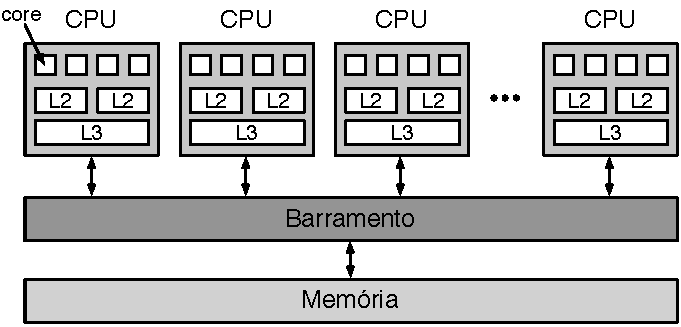
\includegraphics[width=\linewidth]{img/uma}
						\caption{UMA.}
					\end{subfigure}
					\quad\quad
					\begin{subfigure}{0.45\linewidth}
						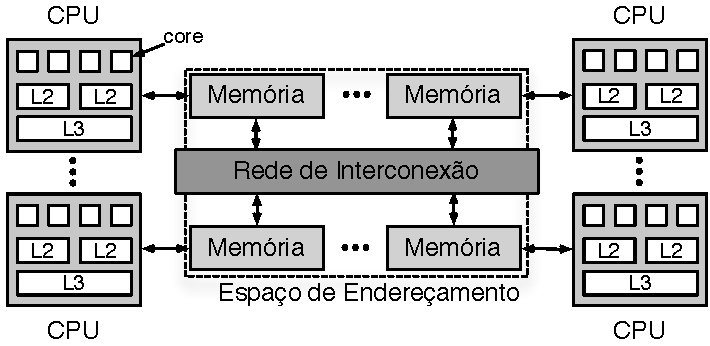
\includegraphics[width=\linewidth]{img/numa}
						\caption{NUMA.}
					\end{subfigure}
				\caption{Exemplos de arquiteturas de memória compartilhada.}
				\label{fig:uma-numa}
			\end{figure}

	Existem duas grandes classes de arquiteturas de memória compartilhada. A
	principal diferença entre elas está relacionado ao tempo de acesso dos
	processadores à memória principal. Em arquiteturas do tipo
	\textit{Uniform Memory Access} (UMA), o tempo de acesso entre o
	processador ou \textit{core} e a memória principal é constante (Figure~\ref{fig:uma-numa}a).
	Por outro lado, em arquiteturas do tipo \textit{Non-Uniform Memory Access}
	(NUMA) o tempo de acesso entre o processador ou \textit{core} não é
	constante (Figura~\ref{fig:uma-numa}b). A diferença no tempo de acesso vem
	do fato de que cada processador ou \textit{core} tem acesso a bancos de memória local
	(próximos a ele) e também a bancos de memória remotos (distantes a ele
	mas próximos de outro processador ou \textit{core}). Nesse sentido, o
	tempo de acesso à memória principal pode ser pequeno (acesso a um banco
	de memória local) ou grande (acesso a um banco de memória remoto),
	dependendo da distância entre o processador ou \textit{core} e o banco
	de memória que esse processador ou \textit{core} está acessando.
	Arquiteturas utilizadas em \textit{notebooks}, \textit{desktops} ou em
	pequenos servidores que contenham poucas dezenas de \textit{cores} são
	do tipo UMA. Porém, arquiteturas paralelas mais complexas que possuem
	várias dezenas de \textit{cores} são normalmente do tipo NUMA.

\section{Conceitos Básicos}

	Essa seção irá abordar os conceitos básicos de programação paralela com
	OpenMP. Primeiramente, será apresentado o modelo base dessa API, em
	seguida será apresentada a diretiva básica para a criação de regiões
	paralelas no código com as formas de compartilhamento de dados
	oferecidas pelo OpenMP.

	\subsection{Modelo Fork-Join}

		% Descrição
		O OpenMP segue o modelo Fork-Join de execução paralela, que é
		ilustrado na Figura~\ref{fig:fork-join}. Nesse modelo, o programa inicia sua
		execução com uma única \textit{thread}, denominada \textit{master thread}
		(Figura~\ref{fig:fork-join}a). A \textit{master thread} executa sequencialmente até
		encontrar uma região paralela, definida pela diretiva \texttt{omp parallel}
		(Figura~\ref{fig:fork-join}b). Nesse ponto, a \textit{master thread} cria um grupo
		de \textit{threads} trabalhadoras, denominadas \textit{worker threads}
		(Figura~\ref{fig:fork-join}c), e cada \textit{worker thread} executa então os
		comandos delimitados pela região paralela. Ao concluírem seu
		trabalho, as \textit{worker threads} sincronizam suas atividades e
		terminam (Figura~\ref{fig:fork-join}d). A \textit{master thread} retoma então a
		execução sequencial do programa até que uma nova região paralela
		seja encontrada, momento em que todo esse processo se repete
		novamente.
		
		% Comentários
		Como observação, é importante deixar claro que a \textit{master
		thread} também executa os comandos na região paralela. Assim, se
		quatro \textit{worker threads} são criadas pela \textit{master
		thread}, um total de cinco \textit{threads} irão executar a região paralela.
		No entanto, é possível fazer uso de estruturas condicionais
		alinhadas a funções internas do OpenMP para definir uma execução de
		comandos diferentes para a \textit{master thread}. Esse assunto será
		abordado mais adiante na Seção \ref{section: sincronizacao}. Por
		fim, vale ressaltar que, em implementações modernas do OpenMP, a
		criação das estruturas internas para gerência das \textit{threads} em regiões
		paralelas é feita uma única vez, quando a primeira região paralela é
		encontrada. Dessa forma, a sobrecarga imposta na aplicação não
		cresce linearmente com o número de regiões paralelas nela presente.

			\begin{figure}[t]
				\centering
				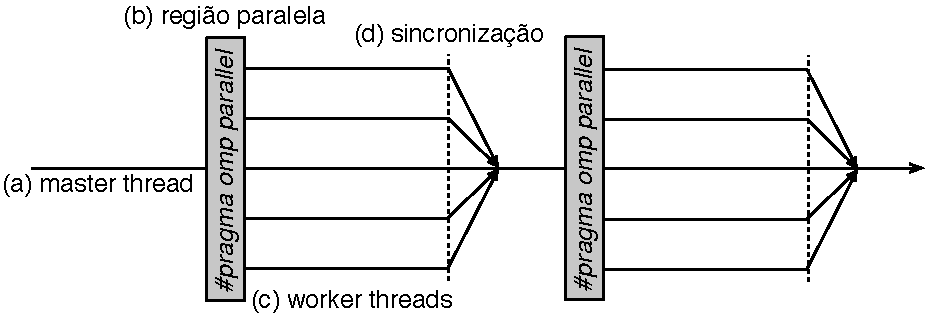
\includegraphics[width=0.8\linewidth]{img/fork-join}
				\caption{Visão geral do modelo Fork-Join.}\label{fig:fork-join}
			\end{figure}

	\subsection{Regiões Paralelas e Compartilhamento de Dados}

		% Descrição.
		A definição de regiões paralelas no OpenMP é feita através da
		diretiva \texttt{omp\_parallel}, como é ilustrado no Código~\ref{listing:sayhello}.
		Nesse exemplo, assim que a a \textit{master thread}
		atinge a região paralela (linhas 7 a 12), ela cria um grupo de
		\textit{worker threads} para executar os comandos especificados. Ao
		final da região paralela, uma barreira implícita força a
		sincronização das \textit{threads}.
		
		% Controle do Número de Threads
		Por padrão, o número de \textit{threads} no grupo que executará uma região
		paralela será igual ao número de núcleos de processamento no
		processador. No entanto, esse fator pode ser controlador através da
		cláusula \texttt{num\_threads()}, pela invocação da função
		utilitária \texttt{omp\_set\_num\_threads()}, ou então pela
		definição da variável de ambiente \texttt{OMP\_NUM\_THREADS}. Em uma região paralela
		as threads são identificadas por um número único entre $0$ e o número total de \textit{threads}$-1$.
		O identificador de cada \textit{thread} pode ser recuperado através da
		função utilitária do OpenMP \texttt{omp\_get\_thread\_num()}.

		% Controle de Escopo de Dados 
		Variáveis declaradas fora da região paralela são compartilhadas entre
		todas as \textit{threads} por padrão. No entanto, a cláusula \texttt{private()}
		pode ser usada para a especificação de variáveis locais privadas, e a
		diretiva \texttt{omp threadprivate} pode ser empregada para a definição
		de variáveis globais privadas. Alternativamente, é possível alterar o
		comportamento padrão para variáveis locais através da cláusula
		\texttt{default()}, definindo todas elas como privadas, e então
		especificar as variáveis locais compartilhadas pela cláusula
		\texttt{shared()}.

		% Programação de Alto Desempenho
		O uso dos mecanismos apresentados anteriormente é fundamental no
		desenvolvimento de aplicações paralelas eficientes. O ajuste do
		número de \textit{threads} em uma região paralela evita o desperdício de
		recursos computacionais e possibilita um ajuste da granularidade de
		tarefas. A identificação de \textit{threads} é necessária para a correta
		coordenação e atribuição de tarefas em uma aplicação. Por fim,
		mecanismos de controle de escopo de dados são inerentemente
		necessários em aplicações paralelas.

\begin{lstlisting}[frame=single, caption=Um exemplo simples com uma região paralela.,
label=listing:sayhello]
void sayhello(int nthreads)
{
	void tids[nthreads]

	/* Cria threads. */
	#pragma omp parallel num_threads(nthreads)
	{
		int tid;

		tid = omp_get_thread_num();
		tids[tid] = tid;
	}

	/* Imprime IDs das threads. */
	for (int i = 0; i < nthreads; i++)
		printf("thread %d: my ID is %d\n", i, tids[i]);
}
\end{lstlisting}

\section{Paralelismo de Dados e Diretivas OpenMP}

	% Visão Geral
	No OpenMP, o paralelismo de dados é explorado através de diretivas
	para paralelização de laços. Nessa seção, o uso dessas diretivas para o
	projeto de aplicações paralelas será discutido.
	Primeiro, serão apresentadas as diretivas que possibilitam explorar o
	paralelismo de dados. Em seguida, as estratégias de escalonamento
	disponíveis no OpenMP são apresentadas, assim como suas vantagens e
	desvantagens. Por fim, os mecanismos de redução oferecidos pela API
	OpenMP são introduzidos.

	\subsection{Paralelização de Laços}
	\label{subsection: paralelização de lacos}

		% Visão Geral
		Duas diretivas de paralelização de laços estão disponíveis no
		OpenMP: \texttt{omp for} e \texttt{omp parallel for}. A primeira
		diretiva instrui que as iterações do laço seguinte de uma região
		paralela devem ser distribuídas entre as \textit{threads} do grupo em questão
		e, então, executadas em paralelo. A segunda diretiva tem o mesmo
		efeito, porém não necessita que o laço esteja dentro de uma região
		paralela. O Código~\ref{listing:matrixmult} ilustra o uso dessa última
		diretiva na paralelização do algoritmo clássico de multiplicação de
		matrizes. Nesse exemplo, um grupo de \textit{threads} é criado para
		executar os comandos do laço da linha $9$. Cada \textit{thread}
		recebe um conjunto distinto de iterações e, assim, a
		computação é efetuada em paralelo. 

\begin{lstlisting}[frame=single, caption=Paralelização da multiplicação de
matrizes no OpenMP.,
, label=listing:matrixmult]
struct matrix *matrix_mult(struct matrix *a, struct matrix *b)
{
	struct matrix *c;

	c = matrix_create(a->nrows, b->ncols);

	/* Multiplica matrizes. */
	#pragma omp parallel for private(i, j, k)
	for (int i = 0; i < a->nrows; i++)
	{
		for (int j = 0; j < a->cols; j++)
		{
			for (int k = 0; k < a->ncols; k++)
				MATRIX(c, i, j) += MATRIX(a, i, k)*MATRIX(b, k, j);
		}
	}

	return (c);
}
\end{lstlisting}

		% Discussão de Granularidade
		Observe que nesse exemplo, assim como em diversas outras aplicações que
		também exploram o paralelismo de dados presente em laços, a diretiva de
		compilação também poderia ter sido colocada no segundo laço mais externo
		sem perda de semântica. No entanto, as duas abordagens se difeririam
		quanto à granularidade de paralelização. Na primeira abordagem, o grão
		de trabalho entregue a cada \textit{thread} é mais grosso, enquanto na segunda
		abordagem o grão de trabalho é mais fino. O controle de granularidade
		consiste em uma técnica importante no projeto de aplicações paralelas
		eficientes, pois possibilita que a localidade temporal e de dados sejam efetivamente
		exploradas além de evitar sobrecargas de sincronização e contornar desbalanceamentos
		de carga durante a computação. Na Seção~\ref{subsection: escalonamento de iteracoes}
		serão discutidas as peculiaridades desse assunto em maiores detalhes.

			\begin{figure}[t]
				\captionsetup[subfigure]{justification=centering}
				\centering
					\begin{subfigure}{0.45\linewidth}
						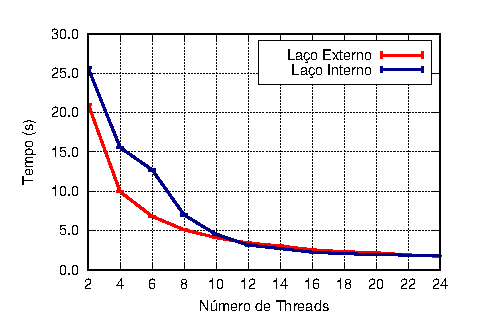
\includegraphics[width=\linewidth]{img/mm}
						\caption{Tempo de execução.}
						\label{figure: time mm}
					\end{subfigure}
					\quad
					\begin{subfigure}{0.45\linewidth}
						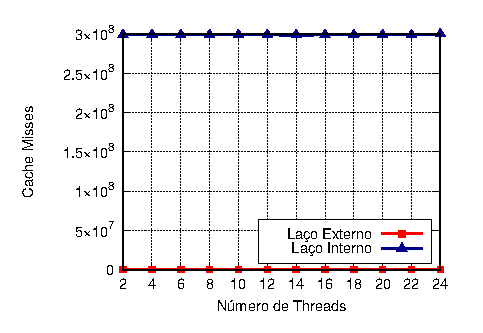
\includegraphics[width=\linewidth]{img/mm-cache}
						\caption{Número de faltas de \textit{cache}.}
						\label{figure: cache misses mm}
					\end{subfigure}
					\caption{Resultados das soluções de paralelização para a
					multiplicação de matrizes.}
			\end{figure}
			
		% Análise de Desempenho
		Para ilustrar o impacto no desempenho que cada uma dessas abordagens
		teriam no algoritmo clássico de multiplicação de matrizes,
		experimentos foram conduzidos em uma máquina SMP com 24 núcleos ($4
		\times$ Xeon X7). Nesses experimentos, o tamanho da matriz de
		entrada foi fixado em $1.680 \times 1.680$, o número de
		\textit{threads} foi variado de $2$ a $24$, e estatísticas de tempo
		de execução e número de faltas na \textit{cache} L2 foram coletadas.
		A análise dos resultados de faltas na \textit{cache} L2 (Figura
		\ref{figure: cache misses mm}) revela que a abordagem de
		paralelização mais grossa conduz a um menor número de faltas, em
		contraste a estratégia de paralelização do laço mais interno, para a
		plataforma e tamanho de problema considerados. Essa diferença conduz
		a um ganho de desempenho que é evidenciado nos resultados de tempo
		de execução da aplicação (Figura \ref{figure: time mm}). Além disso,
		é possível constatar que o ganho obtido com mais que $12$
		\textit{threads} não é significantemente superior do que quando
		menos \textit{threads} são usadas, indicando assim que na
		plataforma considerada o tamanho de problema não escala linearmente
		com o número de \textit{threads}.

	\subsection{Escalonamento de Iterações}
	\label{subsection: escalonamento de iteracoes}

		% Aplicações Regulares
		O escalonamento de iterações diz respeito ao modo como iterações de
		um laço paralelo são atribuídas às \textit{threads} de um grupo. Por padrão,
		no OpenMP, o escalonamento de iterações é feito estaticamente e em
		blocos (ou \textit{chunks}) de mesmo tamanho. Para aplicações que
		possuem um padrão de computação regular, isto é, o tempo de
		computação para cada iteração do laço paralelo é o mesmo, essa
		estratégia conduz a ganhos de desempenhos satisfatórios, pois esse
		particionamento estático é capaz de distribuir a carga de trabalho
		de forma uniforme entre as \textit{threads}. O algoritmo de multiplicação de
		matrizes apresentado na seção anterior exemplifica a classe de
		algoritmos regulares. No caso, a carga de trabalho entregue a cada
		\textit{thread} é constate e proporcional à:
		%
		\begin{equation}
			\text{Carga de Trabalho} = \dfrac{\text{Numéro de Linhas na Matriz}}%
			                                 {\text{Número de Threads}}
		\end{equation}

		
		% Aplicações Irregulares
		No entanto, para aplicações que possuem um caráter irregular de
		computação, isto é, o tempo de computação para cada iteração no laço
		paralelo difere; ou então para aplicações regulares que possuem
		afinidade de memória entre diferentes iterações; essa estratégia não
		se mostra eficiente e escalável~\cite{Carino2008a}. Então, para atacar esses
		cenários problemáticos, o OpenMP disponibiliza a cláusula
		\texttt{schedule()} que possibilita: (i) selecionar a estratégia de
		escalonamento a ser empregada para escalonar as
		iterações de um laço paralelo; e (ii) definir quantas iterações são
		escalonadas por vez a uma única \textit{thread} (\textit{chunk size}).
		A estratégia de escalonamento permite contornar o problema do
		desbalanceamento de carga presente em aplicações irregulares,
		enquanto o controle do tamanho de bloco de iterações a ser escalonado
		por vez permite ajustar a granularidade de paralelização, possibilitando
		assim que a afinidade de memória existente entre iterações seja explorada.
		O tamanho de bloco de iterações pode ser escolhido arbitrariamente,
		já a estratégia de escalonamento pode ser selecionada dentre as
		seguintes, em uma implementação padrão do OpenMP:
		%
		\begin{itemize}
			\item \texttt{static}: particiona igualitariamente as iterações de um
			laço paralelo em \textit{chunks} de iterações. A atribuição de \textit{chunks}
			é feita em tempo de compilação e nenhuma sobrecarga é
			adicionada a aplicação. Essa estratégia é indicada para
			aplicações regulares.
			
			\item \texttt{dynamic}: atribui \textit{chunks} de iterações às \textit{threads} sob
			demanda em tempo de execução. Para que a atribuição seja feita
			dinamicamente durante a execução da aplicação, uma sobrecarga de
			gerência é introduzida na aplicação. Essa estratégia é indicada
			para uso em aplicações com alto grau de irregularidade.

			\item \texttt{guided}: similar à estratégia \texttt{dynamic}, porém o tamanho do
			\textit{chunk} de iterações decresce com o tempo. Essa estratégia
			também impõe uma sobrecarga na execução da aplicação, porém
			relativamente menor que a estratégia \texttt{dynamic}. Essa
			estratégia é indicada para uso em aplicações com baixo e
			médio graus de irregularidade, onde as iterações iniciais
			do laço paralelo podem ser atribuídas em \textit{chunks} maiores, e
			assim alguma sobrecarga de sincronização é evitada durante uma porção
			significativa do tempo total de execução da aplicação.
		\end{itemize}
		
		% Análise de Desempenho
		O Código~\ref{listing:sparsematrixmult} ilustra o uso desses dois
		mecanismos na paralelização do algoritmo clássico para multiplicação
		de matrizes esparsas, um típico representante de uma aplicação
		irregular. Nesse exemplo, o escalonamento de iterações é feito em
		blocos (\textit{chunks}) de tamanho 1 com a política de
		escalonamento \texttt{dynamic}. Uma avaliação quantitativa do
		desempenho dessa estratégia nesse algoritmo particular, frente à
		estratégia \texttt{static}, é apresentada na
		Figura~\ref{fig:static-dynamic-guided}. Os experimentos foram
		conduzidos em uma máquina SMP com 24 cores ($4 \times$ Intel Xeon
		X7 com 6 núcleos cada) para uma matriz de tamanho $1.680 \times 1.680$. 
		O número de \textit{threads} $n$ foi variado de $2$ a $12$ e o tamanho de
		\textit{chunks} foi fixado em $1.680/n$ e $1$, para as estratégias
		escalonamento \texttt{static} e \texttt{dynamic}, respectivamente.
		Para essa aplicação, tamanho de problema e plataforma, a análise dos
		resultados revela que a estratégia de escalonamento \texttt{dynamic}
		conduz a um melhor desempenho do que que a estratégia
		\texttt{static}, se mostrando assim mais escalável.  De fato, esse
		comportamento é recorrente em aplicações irregulares e pode ser
		utilizado para guiar o projeto de soluções paralelas eficientes
		nesse domínio. No entanto, é pertinente observar que a
		granularidade de \textit{chunks} consiste em um fator que impacta
		diretamente no desempenho entregue pela estratégia \texttt{dynamic}
		e, então, deve ser cuidadosamente considerado. 

		% Granularidade de Chunks
		Para enfatizar a influência do tamanho do \textit{chunk} no
		desempenho do escalonador \textit{dynamic}, experimentos com um
		\textit{kernel} sintético que realiza uma computação regular,
		uma soma de um conjunto (grande) de números inteiros, foram
		conduzidos. Diferentes tamanhos de \textit{chunks} foram
		analisados e as estratégias de escalonamento de iterações
		\texttt{static} e \texttt{dynamic} foram consideradas. Os
		resultados obtidos são apresentados na Figura \ref{fig:chunk-size}
		e evidenciam que na estratégia \texttt{dynamic},
		\textit{chunks} muito pequenos introduzem uma expressiva
		sobrecarga na execução, que diminui com o aumento do tamanho do
		\textit{chunk}. Em contraste, a estratégia \texttt{static}
		entrega um desempenho constante à aplicação, independente do
		tamanho do \textit{chunk}.

\begin{lstlisting}[frame=single, caption=Exemplo de multiplicação de matrizes esparsas.,
label=listing:sparsematrixmult]
struct matrix *sparsematrix_mult(struct matrix *a, struct matrix *b)
{
	struct matrix *c;

	c = matrix_create(a->nrows, b->ncols);

	/* Multiplica matrizes esparsas. */
	#pragma omp parallel for private(i, j, k) schedule(dynamic, 1)
	for (int i = 0; i < a->nrows; i++)
	{
		for (int j = 0; j < a->ncols; j++)
		{
			for (int k = 0; k < a->ncols; k++)
			{
				if (MATRIX(a, i, k) != 0)
					MATRIX(c, i, j) += MATRIX(a, i, k)*MATRIX(b, k, j);
			}
		}
	}

	return (c);
}
\end{lstlisting}

		\begin{figure}[t]
			\captionsetup[subfigure]{justification=centering}
			\centering
				\begin{subfigure}{0.45\linewidth}
					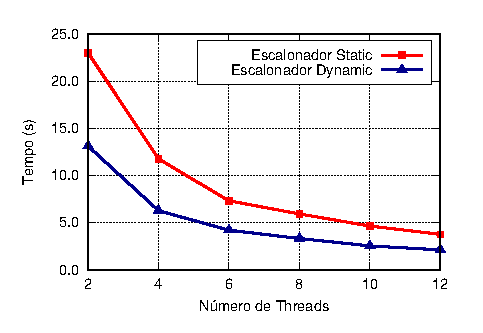
\includegraphics[width=\linewidth]{img/smm}
					\caption{Escalabilidade das estratégias \texttt{dynamic} e \texttt{static}.}
					\label{fig:static-dynamic-guided}
				\end{subfigure}
				\quad
				\begin{subfigure}{0.45\linewidth}
					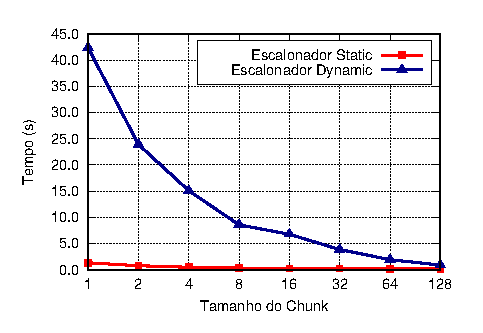
\includegraphics[width=\linewidth]{img/chunk-size}
					\caption{Desempenho para diferentes tamanhos de
					\textit{chunks}.}
					\label{fig:chunk-size}
				\end{subfigure}
			\caption{Desempenho das estratégias \texttt{dynamic} e \texttt{static} obtidos com a versão paralela
			do algoritmo clássico para multiplicação de matrizes esparsas.}
		\end{figure}

	\subsection{Redução de Operações}
	\label{subsection: reducao de operacoes}

		% Visão Geral
		Em aplicações que exploram o paralelismo de dados,
		frequentemente existe uma necessidade de que as \textit{threads}
		combinem seus resultados privados de forma a produzir um
		resultado final para o problema sendo computado. Um suporte
		eficiente a essa operação, denominada redução, é oferecido pelo
		OpenMP através da cláusula \texttt{reduction}. O Código~\ref{listing:prodescalar}
		ilustra o uso da operação de redução para o cálculo
		paralelo do produto escalar de um vetor. Nesse exemplo, cada
		\textit{thread} executa o produto de um subconjunto dos
		elementos do vetor por um escalar e, em seguida, os resultados
		parciais encontrados por cada \textit{thread} são somados, para
		o cálculo do resultado final.

		% Discussão
		Por padrão, o OpenMP oferece suporte  para redução de operações
		aritméticas básicas sobre tipos primitivos da linguagem. Para
		tanto, um cópia privada da variável a ser reduzida é criada em
		cada \textit{thread} e, então, ao final da computação as
		variáveis são combinadas hierarquicamente segundo o operador
		especificado. Para tipos e operadores que o OpenMP não oferece
		suporte, é possível fornecer uma implementação eficiente e
		portável fazendo o uso de um laço paralelo, que efetua a
		computação de interesse, seguido por um laço sequencial que
		realiza a redução dos valores parciais computados.

\begin{lstlisting}[frame=single, caption=Produto escalar.,
label=listing:prodescalar]
int scalar_product(struct vector *a, struct vector *b)
{
	int prod;

	#pragma omp parallel for private(i) schedule (static) reduction(+:prod)
	for (int i = 0; i < a->size; i++)
		prod += VECTOR(a, i) * VECTOR(b, i);
	
	return (prod);
}
\end{lstlisting}


\section{Sincronização}
\label{section: sincronizacao}

	Além de oferecer diretivas úteis para paralelização de porções de código, a API
	OpenMP também oferece diretivas para sincronização de \textit{worker threads}. Essas
	diretivas são utilizadas dentro de regiões paralelas para: (i) indicar a necessidade de serialização
	de um trecho de código; (ii) garantir exclusão mútua ao acesso a dados compartilhados; ou
	(iii) realizar uma sincronização global entre \textit{worker threads}. A seguir, são discutidas
	as principais diretivas de sincronização disponíveis na API OpenMP.
	
	\begin{description}
		\item[\textbf{Serialização.}] A diretiva \texttt{omp single} permite que a execução de um trecho
		de código dentro de uma região paralela seja serializada, ou seja, seja executada por apenas
		uma \textit{worker thread}. O OpenMP implementa uma ou diretiva similar para serialização
		de trechos de código denominada \texttt{omp master}. A diferença entre as primitivas \texttt{omp single}
		e \texttt{omp master} reside no fato de que, na primeira, qualquer \textit{worker thread} pode executar
		o trecho de código serializado, ao passo que, na segunda, somente a \textit{master thread} executará
		o trecho de código serializado.
		
		\item[\textbf{Exclusão mútua.}] Em muitos casos, dados compartilhados necessitam modificados dentro
		de uma região paralela por todas as \textit{worker threads}. Nesses trechos de código, denominados
		\textit{seções críticas}, faz-se necessária a utilização e um mecanismo de exclusão mútua para evitar
		que duas ou mais \textit{worker threads} tenham acesso simultaneamente aos dados compartilhados.
		Para esses casos, a API OpenMP oferece duas diretivas principais. A primeira delas, denominada
		\texttt{omp critical}, implementa um mecanismo de exclusão mútua clássico com uso de \textit{locks}
		similar ao \textit{mutex}. A segunda delas, denominada \texttt{omp atomic}, é semelhante à primeira, 
		porém somente pode ser utilizada para proteger operações simples sobre uma variável compartilhada.
		Por exemplo, para uma variável compartilhada \texttt{x}, as operações permitidas pela diretiva
		\texttt{omp atomic} são: (i) \textbf{leitura}, e.g., \texttt{v = x}; (ii) \textbf{escrita}, e.g., \texttt{x =} \textit{expr}
		(onde \textit{expr} é uma expressão aritmética); (iii) \textbf{atualização}, e.g., \texttt{x++}; ou (iv) 
		\textbf{incremento/decremento}, e.g., \texttt{v = x++}. A lista completa de operações permitidas está
		disponível na especificação OpenMP\footnote{Disponível em \url{http://openmp.org/wp/openmp-specifications/}}.
		É importante notar que, para o caso de uma seção crítica contendo uma única operação aritmética,
		amas as diretivas podem ser utilizadas. Porém, nesse caso, a diretiva \texttt{omp atomic} oferecerá
		um melhor desempenho, pois a sua implementação utiliza \textit{spin-locks} e instruções de \textit{hardware}
		para garantir a atomicidade das operações.
		
		\item[\textbf{Sincronização global.}] O OpenMP também oferece uma diretiva que permite realizar uma
		sincronização global entre as \textit{worker threads} na forma de uma \textit{barreira}. Essa primitiva,
		denominada \texttt{omp barrier}, garante que todas as \textit{worker threads} somente possam executar
		as instruções posteriores à barreira quando todas as \textit{worker threads} tiverem chegado a ela.
	\end{description}
	
	Na seção seguinte também será discutida uma diretiva de sincronização específica para o paralelismo de tarefas.

\section{Paralelismo de Tarefas e Diretivas OpenMP}

	A partir da versão 3.0 foi introduzido o conceito de tarefas (\textit{tasks}) no OpenMP.
	No OpenMP a criação de tarefas pode ser feita por uma ou mais \textit{threads}. Ao
	serem criadas, as tarefas que ainda não foram computadas são inseridas em uma
	estrutura de dados compartilhada entre as \textit{threads} denominada ``saco de tarefas''
	(\textit{bag of tasks}). Dentro de uma região paralela, ao ficarem ociosas, as \textit{threads}
	retiram tarefas ainda não computadas do saco de tarefas e as processam uma a uma.
	
	A Figura~\ref{fig:tasks} apresenta uma visão geral do modelo de tarefas implementado
	no OpenMP. Nesse exemplo, algumas \textit{threads} somente criam tarefas (representadas
	por flechas unidirecionais com linhas tracejadas) enquanto outras somente executam tarefas
	(representadas por flechas unidirecionais com linhas pontilhadas). É permitido também que,
	ao executar uma tarefa, uma \textit{thread} possa criar novas tarefas (representadas por
	flechas bidirecionais com linhas contínuas). A possibilidade de uma tarefa criar novas tarefas
	permite que o algoritmo a ser paralelizado possa ser recursivo.
	
		\begin{figure}[t]
			\centering
			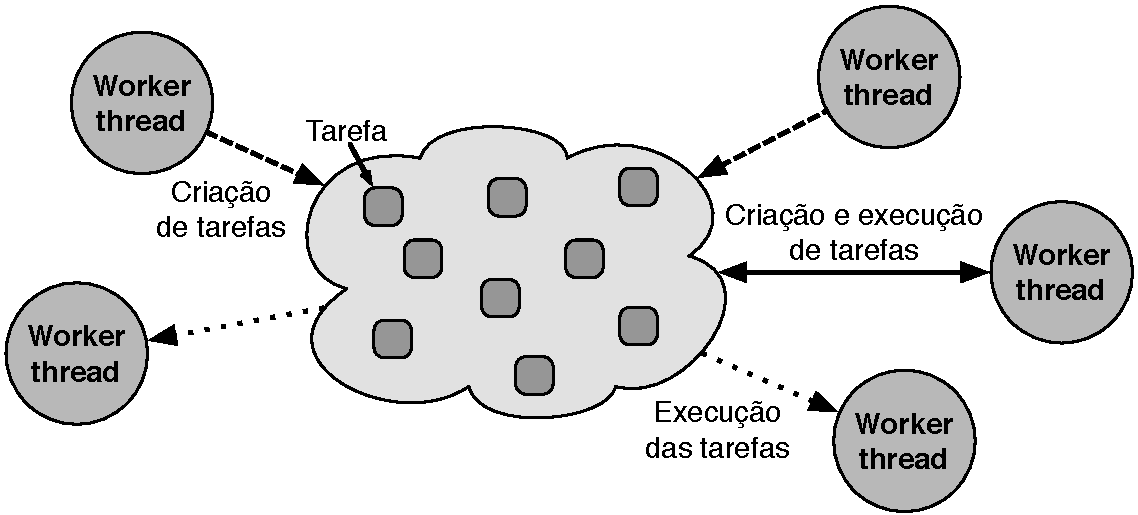
\includegraphics[width=0.6\linewidth]{img/tasks}
			\caption{Paralelismo de tarefas do OpenMP: uma ou mais \textit{threads} criam
			tarefas, as quais são inseridas em uma estrutura de dados compartilhada
			que contém tarefas ainda não computadas. \textit{Threads} ociosas em
			uma região paralela retiram tarefas dessa estrutura e as processam uma a
			uma.}
			\label{fig:tasks}
		\end{figure}

	A criação e execução de tarefas pelas \textit{threads} é sempre feita dentro de uma região paralela
	criada com o uso da diretiva \texttt{omp parallel}. Dentro de uma região paralela, \textit{threads} podem
	criar tarefas a serem computadas através do uso da diretiva \texttt{omp task}. Quando uma tarefa é criada,
	a mesma é inserida no saco de tarefas e fica disponível para ser computada por qualquer \textit{worker thread}
	ociosa dentro da região paralela.

	Em muitos problemas computacionais paralelizados com o uso de tarefas, determinadas tarefas não podem
	ser computadas pois dependem de resultados de outras tarefas ainda não finalizadas. Essas dependencias
	podem ser vistas na forma de um grafo direcionado de dependências, onde cada nó do grafo representa
	uma tarefa e as arestas representam as dependências entre elas. A dependência entre tarefas é determinada
	no OpenMP através da diretiva \texttt{omp taskwait}. Essa diretiva permite que uma instrução ou um bloco de
	instruções em uma tarefa só seja executado após o término de todas as tarefas criadas anteriormente.
	
	Um exemplo clássico de um problema recursivo que pode ser paralelizado com o uso de tarefas é a soma da
	sequência de Fibonacci. Matematicamente, os números da sequência de Fibonacci são gerados através da
	seguinte fórmula recursiva:
	
	\begin{equation}
		F_n = F_{n-1} + F_{n-2} \text{, onde } F_1=1 \text{ e } F_2=1
	\end{equation}

	Se considerarmos que para calcular $F_n$ são necessárias duas tarefas $F_{n-1}$ e $F_{n-2}$, é evidente que
	os resultados de $F_{n-1}$ e $F_{n-2}$ só poderão ser somados após o término de ambas tarefas. Nesse caso,
	nota-se que $F_n$ depende de $F_{n-1}$ e $F_{n-2}$. A Figura~\ref{fig:fibonacci} mostra um exemplo de um
	grafo de dependências de tarefas para o cálculo da soma da sequência de Fibonacci usando tarefas. Nesse
	exemplo, cada tarefa representa uma chamada recursiva à $F_{n-1}$ e $F_{n-2}$.

		\begin{figure}[t]
			\centering
			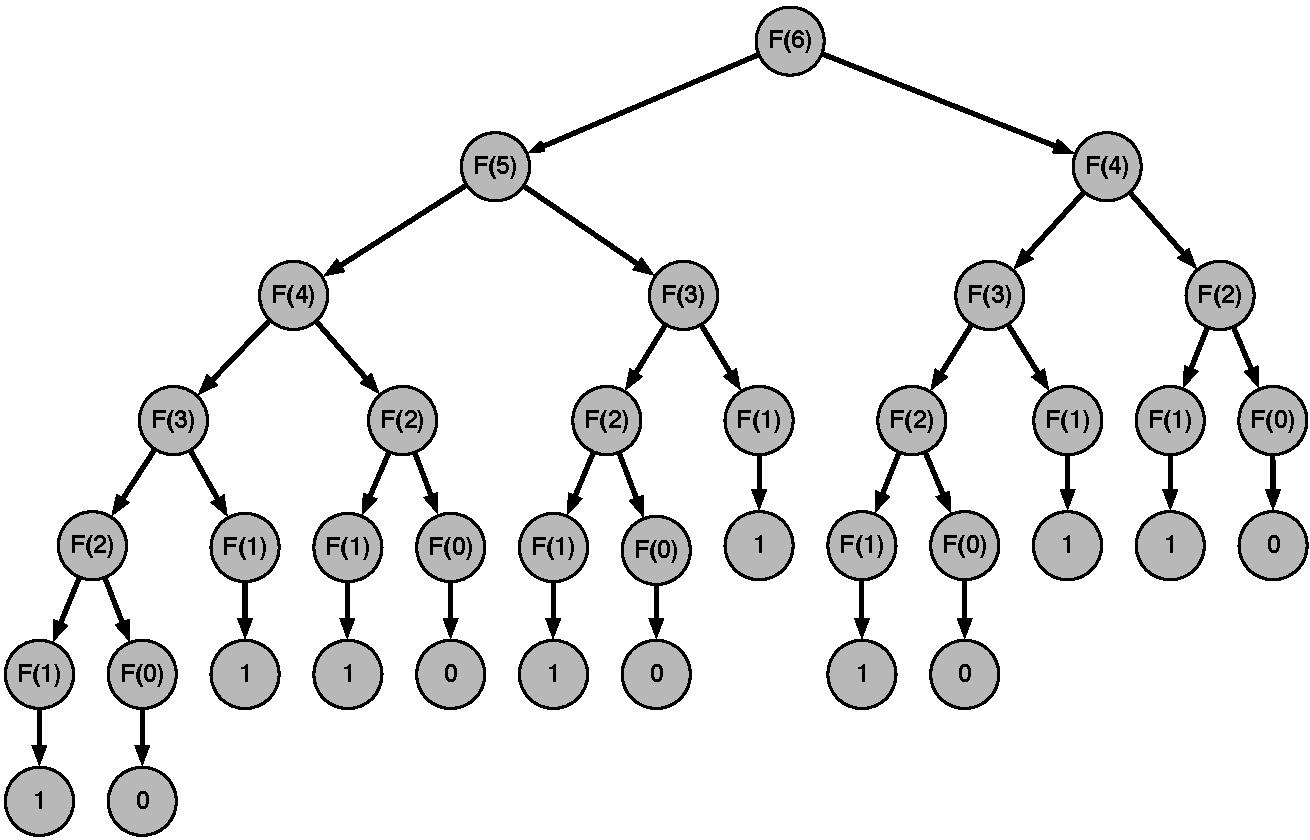
\includegraphics[width=0.8\linewidth]{img/fibonacci}
			\caption{Grafo de dependência de tarefas gerado pelo algoritmo que calcula a soma da sequência
			de Fibonacci.}\label{fig:fibonacci}
		\end{figure}

	O Código~\ref{listing:fibonacci} mostra um exemplo de implementação básica para o cálculo da soma da sequência
	de Fibonacci usando tarefas em OpenMP. Primeiramente é criada uma região paralela com o uso da diretiva
	\texttt{omp parallel} (linha 5). Para permitir que somente uma única \textit{worker thread} inicie a computação, e
	consequentemente, a criação das primeiras tarefas, utiliza-se a diretiva \texttt{omp single} (linha 7). A primeira
	\textit{worker thread} que ganhar acesso à região \texttt{omp single} executa uma chamada à função recursiva 
	\texttt{recursive\_fibonacci()}. A cláusula \textit{nowait} permite que as demais \textit{worker threads} avancem até
	a barreira implícita ao final da região paralela. Na função \texttt{recursive\_fibonacci()}, tarefas correspondentes ao
	cálculo $F_{n-1}$ e $F_{n-2}$ são criadas com o uso da diretiva \texttt{omp task} (linhas 27--28 e 30--31) assim
	como as dependências são criadas com a diretiva \texttt{omp taskwait} (linhas 33--34).
	
	Note que o Código~\ref{listing:fibonacci} inclui uma condição de parada específica para a criação de tarefas (linha 23),
	evitando-se explicitamente a criação de tarefas quando o valor da variável \texttt{n} é inferior a um valor específico (\texttt{stop}). 
	Basicamente, essa condição garante uma carga \textit{mínima} para computação de uma tarefa. Em outras palavras, a
	computação será realizada sequencialmente por cada \textit{worker thread} quando \texttt{n < stop}. Portanto,
	a variável \texttt{stop} pode ser vista como uma forma de controle de granularidade das tarefas da aplicação.
	A condição de parada para criação de tarefas é muito importante, tendo em vista que a criação e gestão de tarefas no
	OpenMP possui um sobrecusto significativo. Logo, é importante que as tarefas tenham uma carga grande o suficiente de forma
	a reduzir o sobrecusto anteriormente mencionado. Todavia, tarefas contendo cargas extremamente grandes podem gerar
	desbalanceamentos de carga entre as \textit{worker threads}.

\begin{lstlisting}[frame=single, caption=Exemplo de uma implementação recursiva simples da soma da sequencia de Fibonacci
usando tarefas., label=listing:fibonacci]
int fibonacci(int n, int stop)
{
	int result;
	
	#pragma omp parallel
  	{
		#pragma omp single nowait
		result = recursive_fibonacci(n, stop);
	}
		
	return (result);
}

long recursive_fibonacci(int n, int stop)
{
	long f1, f2, fn;

	/* Condicao de parada da recursao. */
	if (n == 0 || n == 1) 
		return (n);

	/* Condicao de parada da criacao de tarefas. */
	if (n < stop) 
		return (recursive_fibonacci(n-1, stop) + recursive_fibonacci(n-2, stop));
	else
	{	/* Criacao de tarefas e suas dependencias. */
		#pragma omp task shared(f1)
		f1 = recursive_fibonacci(n-1, stop);

		#pragma omp task shared(f2)
		f2 = recursive_fibonacci(n-2, stop);
		
		#pragma omp taskwait
		fn = f1 + f2;
			
		return (fn);
	}
}
\end{lstlisting}

	Uma avaliação do impacto da granularidade das tarefas no desempenho da aplicação é apresentada na
	Figura~\ref{fig:grao-tarefas}. Os experimentos foram conduzidos em uma máquina SMP com 24 cores
	($4 \times$ Intel Xeon X7 com 6 núcleos cada). Nesses experimentos, o número de \textit{threads} foi fixado
	em 12 e o valor da variável \texttt{n} foi fixado em 50.

%	\begin{figure}[t]
%		\centering
%		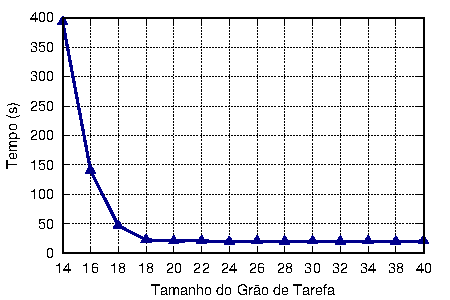
\includegraphics[width=8cm, height=!]{img/fibonacci-task-grain}
%		\caption{Impacto da granularidade das tarefas no desempenho do cálculo da soma da sequência
%		de Fibonacci.}
%		\label{fig:grao-tarefas}
%	\end{figure}

\section{Conclusão}

	Esse capítulo apresentará um apanhado geral do minicurso, ressaltando os
	principais pontos abordados no texto.

\bibliography{referencias}

\end{document}
